% Options for packages loaded elsewhere
\PassOptionsToPackage{unicode}{hyperref}
\PassOptionsToPackage{hyphens}{url}
\PassOptionsToPackage{dvipsnames,svgnames,x11names}{xcolor}
%
\documentclass[
  letterpaper,
  DIV=11,
  numbers=noendperiod]{scrartcl}

\usepackage{amsmath,amssymb}
\usepackage{iftex}
\ifPDFTeX
  \usepackage[T1]{fontenc}
  \usepackage[utf8]{inputenc}
  \usepackage{textcomp} % provide euro and other symbols
\else % if luatex or xetex
  \usepackage{unicode-math}
  \defaultfontfeatures{Scale=MatchLowercase}
  \defaultfontfeatures[\rmfamily]{Ligatures=TeX,Scale=1}
\fi
\usepackage{lmodern}
\ifPDFTeX\else  
    % xetex/luatex font selection
\fi
% Use upquote if available, for straight quotes in verbatim environments
\IfFileExists{upquote.sty}{\usepackage{upquote}}{}
\IfFileExists{microtype.sty}{% use microtype if available
  \usepackage[]{microtype}
  \UseMicrotypeSet[protrusion]{basicmath} % disable protrusion for tt fonts
}{}
\makeatletter
\@ifundefined{KOMAClassName}{% if non-KOMA class
  \IfFileExists{parskip.sty}{%
    \usepackage{parskip}
  }{% else
    \setlength{\parindent}{0pt}
    \setlength{\parskip}{6pt plus 2pt minus 1pt}}
}{% if KOMA class
  \KOMAoptions{parskip=half}}
\makeatother
\usepackage{xcolor}
\setlength{\emergencystretch}{3em} % prevent overfull lines
\setcounter{secnumdepth}{5}
% Make \paragraph and \subparagraph free-standing
\ifx\paragraph\undefined\else
  \let\oldparagraph\paragraph
  \renewcommand{\paragraph}[1]{\oldparagraph{#1}\mbox{}}
\fi
\ifx\subparagraph\undefined\else
  \let\oldsubparagraph\subparagraph
  \renewcommand{\subparagraph}[1]{\oldsubparagraph{#1}\mbox{}}
\fi


\providecommand{\tightlist}{%
  \setlength{\itemsep}{0pt}\setlength{\parskip}{0pt}}\usepackage{longtable,booktabs,array}
\usepackage{calc} % for calculating minipage widths
% Correct order of tables after \paragraph or \subparagraph
\usepackage{etoolbox}
\makeatletter
\patchcmd\longtable{\par}{\if@noskipsec\mbox{}\fi\par}{}{}
\makeatother
% Allow footnotes in longtable head/foot
\IfFileExists{footnotehyper.sty}{\usepackage{footnotehyper}}{\usepackage{footnote}}
\makesavenoteenv{longtable}
\usepackage{graphicx}
\makeatletter
\def\maxwidth{\ifdim\Gin@nat@width>\linewidth\linewidth\else\Gin@nat@width\fi}
\def\maxheight{\ifdim\Gin@nat@height>\textheight\textheight\else\Gin@nat@height\fi}
\makeatother
% Scale images if necessary, so that they will not overflow the page
% margins by default, and it is still possible to overwrite the defaults
% using explicit options in \includegraphics[width, height, ...]{}
\setkeys{Gin}{width=\maxwidth,height=\maxheight,keepaspectratio}
% Set default figure placement to htbp
\makeatletter
\def\fps@figure{htbp}
\makeatother
% definitions for citeproc citations
\NewDocumentCommand\citeproctext{}{}
\NewDocumentCommand\citeproc{mm}{%
  \begingroup\def\citeproctext{#2}\cite{#1}\endgroup}
\makeatletter
 % allow citations to break across lines
 \let\@cite@ofmt\@firstofone
 % avoid brackets around text for \cite:
 \def\@biblabel#1{}
 \def\@cite#1#2{{#1\if@tempswa , #2\fi}}
\makeatother
\newlength{\cslhangindent}
\setlength{\cslhangindent}{1.5em}
\newlength{\csllabelwidth}
\setlength{\csllabelwidth}{3em}
\newenvironment{CSLReferences}[2] % #1 hanging-indent, #2 entry-spacing
 {\begin{list}{}{%
  \setlength{\itemindent}{0pt}
  \setlength{\leftmargin}{0pt}
  \setlength{\parsep}{0pt}
  % turn on hanging indent if param 1 is 1
  \ifodd #1
   \setlength{\leftmargin}{\cslhangindent}
   \setlength{\itemindent}{-1\cslhangindent}
  \fi
  % set entry spacing
  \setlength{\itemsep}{#2\baselineskip}}}
 {\end{list}}
\usepackage{calc}
\newcommand{\CSLBlock}[1]{\hfill\break#1\hfill\break}
\newcommand{\CSLLeftMargin}[1]{\parbox[t]{\csllabelwidth}{\strut#1\strut}}
\newcommand{\CSLRightInline}[1]{\parbox[t]{\linewidth - \csllabelwidth}{\strut#1\strut}}
\newcommand{\CSLIndent}[1]{\hspace{\cslhangindent}#1}

\KOMAoption{captions}{tableheading}
\makeatletter
\@ifpackageloaded{caption}{}{\usepackage{caption}}
\AtBeginDocument{%
\ifdefined\contentsname
  \renewcommand*\contentsname{Table of contents}
\else
  \newcommand\contentsname{Table of contents}
\fi
\ifdefined\listfigurename
  \renewcommand*\listfigurename{List of Figures}
\else
  \newcommand\listfigurename{List of Figures}
\fi
\ifdefined\listtablename
  \renewcommand*\listtablename{List of Tables}
\else
  \newcommand\listtablename{List of Tables}
\fi
\ifdefined\figurename
  \renewcommand*\figurename{Figure}
\else
  \newcommand\figurename{Figure}
\fi
\ifdefined\tablename
  \renewcommand*\tablename{Table}
\else
  \newcommand\tablename{Table}
\fi
}
\@ifpackageloaded{float}{}{\usepackage{float}}
\floatstyle{ruled}
\@ifundefined{c@chapter}{\newfloat{codelisting}{h}{lop}}{\newfloat{codelisting}{h}{lop}[chapter]}
\floatname{codelisting}{Listing}
\newcommand*\listoflistings{\listof{codelisting}{List of Listings}}
\makeatother
\makeatletter
\makeatother
\makeatletter
\@ifpackageloaded{caption}{}{\usepackage{caption}}
\@ifpackageloaded{subcaption}{}{\usepackage{subcaption}}
\makeatother
\ifLuaTeX
  \usepackage{selnolig}  % disable illegal ligatures
\fi
\IfFileExists{bookmark.sty}{\usepackage{bookmark}}{\usepackage{hyperref}}
\IfFileExists{xurl.sty}{\usepackage{xurl}}{} % add URL line breaks if available
\urlstyle{same} % disable monospaced font for URLs
\hypersetup{
  pdftitle={The war on drugs is a war on us - young people who use drugs and the fight for harm reduction in the Global South},
  pdfauthor={MJ Stowe; Rita Gatonye; Ruby Lawlor; Ishwor Mahajan; Seyi Kehinde; Sidarth Arya; Jorge Herrera Valderrábano; Angela Mcbride; Florian Scheibein; Emmy Kageha Igonya; Danya Fast},
  pdfkeywords={Youth, Global South, Young people who use drugs, Harm
Reduction},
  colorlinks=true,
  linkcolor={blue},
  filecolor={Maroon},
  citecolor={Blue},
  urlcolor={Blue},
  pdfcreator={LaTeX via pandoc}}

\title{The war on drugs is a war on us - young people who use drugs and
the fight for harm reduction in the Global South}
\author{MJ Stowe \and Rita Gatonye \and Ruby Lawlor \and Ishwor
Mahajan \and Seyi Kehinde \and Sidarth Arya \and Jorge Herrera
Valderrábano \and Angela Mcbride \and Florian Scheibein \and Emmy Kageha
Igonya \and Danya Fast}
\date{2023-11-18}

\begin{document}
\maketitle
\begin{abstract}
In the Global South, young people who use drugs (YPWUD) are exposed to
multiple interconnected social and health harms, with many low- and
middle-income countries enforcing racist, prohibitionist-based drug
policies that generate physical and structural violence and oppression.
While harm reduction coverage for YPWUD is suboptimal globally, in low-
and middle-income countries youth-focused harm reduction services are
particularly lacking. Harm reduction programs in these countries are
often powerfully shaped by global health funding regimes that restrict
progressive programming and reach. In this commentary we highlight the
efforts of young people, activists, allies, and organisations across
some Global South settings to enact programs such as those focused on
peer-to-peer information sharing and advocacy, overdose monitoring and
response, and drug checking. We draw on our experiential knowledge and
expertise to identify and discuss key challenges, opportunities, and
recommendations for youth harm reduction movements, programs and
practices in low- to middle-income countries and beyond, focusing on the
need for youth-driven interventions. We conclude this commentary with
several calls to action to advance harm reduction for YPWUD within and
across Global South settings.
\end{abstract}
\subsection{Introduction}\label{introduction}

In the Global South, young people are often exposed to multiple
interconnected social and health harms as a result of the war on drugs
(Stockings et al. 2016; Degenhardt et al. 2016; Kimmel et al. 2020),
with many low- and middle-income countries imposing racist, classist,
and prohibitionist drug policies through a continuum of violence that
encompasses physical and structural assaults (Daniels et al. 2021;
Tinasti 2018; Duarte, Salas-Hernández, and Griffin 2020). Young people
who use drugs (YPWUD) in the context of various intersections of age,
race, class, gender, sexuality, mental health challenges, and
involvement in criminalized income generation activities such as sex
work often experience heightened violence and oppression and worse
health and social outcomes (Jacobs et al. 2020; Torre-Luque, Ozeylem,
and Essau 2021; Tinasti 2018; Krug, Hildebrand, and Sun 2015). Despite
increasing global coverage of harm reduction services, there remains a
lack of youth-focused harm reduction services, especially in low- and
middle-income countries (Colledge-Frisby et al. 2023). In general,
across these settings, public health systems are often characterized by
systemic under investment and deteriorating infrastructures, human
resource crises, and corruption (Serebryakova, Cook, and Davies 2021).
Conflicting public health, international donor funding, and law
enforcement agendas impede the implementation of many evidence-based
harm reduction programs. The criminalization and moralization of drugs
and the people who use them powerfully undermines access to those harm
reduction services that do exist (Wodak 2012; Toumbourou et al. 2007).
In places where it is possible to access harm reduction programs
(usually run by non-governmental organizations), YPWUD are
disproportionately underserved relative to older populations in these
contexts (Ogundipe et al. 2018; Krug 2012).

Across the Global South, the war on drugs is too often a violent,
racist, and classist war on YPWUD in the context of multiple and
intersecting forms of oppression and limited access to care (Daniels et
al. 2021) . Yet, YPWUD as well as youth-led and youth-inclusive
organizations in these settings are actively pioneering harm reduction
programs to meet their needs and the needs of their communities (Canêdo
et al. 2022). This commentary is authored by YPWUD -- past and present
-- from countries throughout the Global South, alongside academic and
community allies from low- and middle-income countries as well as higher
income countries. We are a heterogeneous group, yet each of us embraces
harm reduction as a set of ideological principles and pragmatic
strategies rooted in social and health justice and a commitment to human
rights, including the right to health for all people (Pauly 2008). We
believe that harm reduction is characterised by an absence of judgement
towards drug use and respect for an individual's choice to use drugs
(Zampini 2018). Since 2009, the World Health Organisation has provided a
list of harm reduction interventions for the prevention, treatment and
care of people who inject drugs and are living with or at risk of HIV,
including needle distribution and exchange programs, opioid agonist
therapy, and HIV testing and treatment programs (World Health
Organization et al. 2009). However, we argue that harm reduction
programming for people who use drugs, including YPWUD, must extend
beyond HIV prevention, testing and treatment. Programming must include
interventions such as the distribution of a range of supplies (not just
needles -- for example, safer smoking kits), take-home naloxone
programs, drug checking services, drug consumption spaces, and peer-led
information sharing, support, and advocacy. Unfortunately, across many
Global South settings, donor funding has been insufficient to support
this kind of comprehensive harm reduction programming, including for
YPWUD (Serebryakova, Cook, and Davies 2021). We have therefore taken
matters into our own hands, in some cases despite tremendous risks to
our safety and the safety of our communities.

The purpose of this commentary is to further ignite much needed
conversations about YPWUD and harm reduction in the Global South. It
centres the diverse efforts of young people, activists, allies, and
organisations across numerous Global South settings to enact programs
such as those focused on peer-to-peer information sharing and advocacy,
overdose monitoring and response, and drug checking. This is by no means
a comprehensive overview of what is happening when it comes to YPWUD and
harm reduction in the Global South. So many success stories are missing
from what follows, in part because we struggled to connect -- and stay
connected with -- young drug user activists and harm reduction
practitioners across the globe. These young people are oftentimes
overworked, overwhelmed, and under compensated as they attempt to keep
themselves and their communities safe while under the weight of poverty,
the drug war, and other forms of oppression. They may be completely new
to these kinds of scholarly outputs, and lack access to mentors who are
able assist with the challenging work of writing (often in a second
language). The timeline of this kind of work can also be frustrating; a
large investment of time and energy is required, but the rewards of
contributing are unclear, especially as time passes and a publication
has still not come to fruition. Sharing a number of the harm reduction
success stories that we were able to collect, we draw on our
experiential knowledge and expertise to identify and discuss key
challenges, opportunities, and recommendations for youth harm movements,
programs and practices in low- to middle-income countries and beyond,
focusing on the need for youth-driven healthcare and harm reduction
interventions.

\subsection{A note on language}\label{sec-language}

There are major limitations to the language of both ``young people who
use drugs (YPWUD)'' and the ``Global South'' that we employ throughout
this commentary. Both terms may ultimately obscure more than they
reveal, because they often seem to place finite boundaries around what
in reality are much messier social and geographic categories.
Definitions of ``young people'' and ``youth'' -- and lived experiences
of these categories -- vary widely across settings and contexts, where
intersections of age, gender, sexual orientation, class, race, human
immunodeficiency virus (HIV) status, and other dimensions of
positionality are mediated by particular configurations of power and
political economy to shape these social categories and lived experiences
(Duarte, Salas-Hernández, and Griffin 2020). Does it make sense to talk
about young people and youth as those under twenty-four or twenty-nine
years of age, when many individuals continue to strongly identify with
these categories -- and with youth drug user activism and movements --
well into their thirties, often due to entrenched, shared circumstances
of precarity as well as shared visions for possible solutions (Canêdo et
al. 2022; Stowe et al. 2022)? Conversely, do age-definitions of young
people and youth make sense when referring to those for whom poverty,
lack of education, unemployment, violence, migration, HIV, and other
difficulties have forced them to move directly from childhood to
adulthood, without the possibility of experiencing youth as a period of
transition or activism and power (D'Ambruoso et al. 2022)? Similarly, it
may not make sense to talk about a Global South composed of countries
and regions in Africa, Latin America, and parts of Asia that meet
certain criteria according to the World Bank income-per-capita index,
when many so-called ``Global North'' settings are home to populations
experiencing similar levels of entrenched poverty and structural
oppression, also as a result of historical and ongoing processes of
colonialism and capitalism (Buxton 2020). Recognizing the limitations of
this language, in this commentary we have chosen to use the term Global
South (rather than listing out a number of discrete countries and
regions in various instances) in order to emphasize some of the common
and disproportionate impacts of the war on drugs on YPWUD across low-
and middle-income countries (Buxton 2020). We use the term young people
to mark ourselves out as a unique demographic with specific harm
reduction priorities, needs, and desires that is simultaneously
characterized by fluidity of meaning and association not necessarily
determined by numerical age.

\subsection{Shared Challenges}\label{sec-challenges}

There is a severe lack of data on the situation of YPWUD in the Global
South (Doyle et al. 2022). What we do know is that those between the
ages of 14 and 34 account for more than one third of the population in
low-income countries, and rates of substance use are high and climbing
among this age range(Jumbe et al. 2021; David, Wegner, and Majee 2023).
YPWUD in the Global South are vulnerable to a myriad of social and
health harms (exacerbated by the COVID-19 pandemic), including
blood-borne infections (e.g.~HIV, HCV), fatal and non-fatal opioid
involved overdose, skin and soft tissue infections, police violence and
extrajudicial murder and mass incarceration (Jumbe et al. 2021;
Degenhardt et al. 2016; Hall et al. 2016; Scheim et al. 2020).

Global coverage of harm reduction interventions is suboptimal , but this
is particularly the case in lower- and middle-income countries
(Colledge-Frisby et al. 2023). For example, the Global State of Harm
Reduction Report (Harm Reduction International 2020) highlights that
only fourteen out of twenty-five countries or regions in these parts of
the world have existing needle exchange programs. Countries or regions
that do have needle exchange programs generally also provide opioid
agonist therapy, such as methadone. However, even in these settings,
life-saving interventions such as drug consumption spaces and take-home
naloxone programs remain largely unavailable (Colledge-Frisby et al.
2023).

Across Global South settings, YPWUD and the organizations they are a
part of face particularly dire challenges in implementing much needed
harm reduction services due to hostile and militarized governments,
systemic corruption, violent policing, punitive laws and forced
treatment or rehabilitation models, precarious and conditional state and
international funding, and entrenched stigma and oppression (D'Ambruoso
et al. 2022; Des Jarlais et al. 2013; Krug 2012). High levels of
unemployment, poverty, and homelessness often combine with the
criminalization of drug use (in some cases via the death penalty and
extrajudicial killings), sex work, and sexual and gender identities to
produce egregious human rights violations and make harm reduction
organising and action difficult, and sometimes impossible (D'Ambruoso et
al. 2022; DeBeck et al. 2017; Rekart 2005). In a system of prohibition,
the Global South is also disproportionately impacted by the various
negative effects of the global demand for illicit drugs, which
particularly impacts countries in Latin America, South East Asia and the
Middle East and North Africa, as well as in transit regions such as West
Africa (UNODC 2022).

\subsection{Success Stories}\label{sec-success}

While significant challenges remain for implementing comprehensive harm
reduction programming for YPWUD across Global South settings (Daniels et
al. 2021; Chang et al. 2021), several of us are actively involved in
implementing various harm reduction programs in our countries. We share
these examples here with the goal of inspiring youth drug user activism
and meaningful policy and programming change across lower- and
middle-income settings globally.

\subsection{East Africa}

\subsubsection{Empowering young women who use drugs in East Africa
through online networking and peer
support}\label{empowering-young-women-who-use-drugs-in-east-africa-through-online-networking-and-peer-support}

A majority of empowerment efforts directed towards women who use drugs
are under-resourced, patriarchal, or fail to consider how complex
intersections of age, gender, class, cultural, and geographic contexts
shape drug use (Lambdin et al. 2013). In 2022, the community-led
organization Women in Response to HIV/AIDS and Drug Addiction (WRADA)
set out to build a network of young women who use drugs in Kenya, Uganda
and Tanzania with support from the International Network of People who
use Drugs. This multi-year community initiative involves bi-monthly
online peer support forums using Zoom. Young women meet on Zoom to
discuss and document regional harm reduction challenges and emerging
trends in drug use and sex work and develop sexual and reproductive
health and harm reduction information tailored to their communities. The
project fosters empowerment by increasing the knowledge, skills and
capacities of participants, growing grassroots harm reduction research
and advocacy, developing context-driven approaches to promoting human
rights, and providing peer mental health support. Despite challenges
with internet connectivity and technological know-how among
participants, the project has resulted in improved relationships between
young women who use drugs and local harm reduction programs across East
Africa, greater advocacy for adoption of best practices through a
peer-to-peer learning model, the generation of more robust evidence for
regional harm reduction and drug policy reform, and increased visibility
of young women who use drugs in East Africa.

\subsection{South Africa}

\subsubsection{Distributing take-home naloxone kits and overdose
education in South
Africa}\label{distributing-take-home-naloxone-kits-and-overdose-education-in-south-africa}

In South Africa, YPWUD are an underserved population frequently exposed
to the social and health harms of HIV and HCV incidence, skin and
soft-tissue infection, poverty, unstable housing and homelessness, and
multiple forms of physical and structural violence (D'Ambruoso et al.
2022; Peltzer and Phaswana-Mafuya 2018). Heroin use and overdose are
increasingly common among youth (Harker et al. 2020). While South
Africa's essential medicines list includes naloxone for the management
of overdose, to date no state-sponsored naloxone distribution programmes
exist (Scheibe, Shelly, and Versfeld 2020). To improve access to this
lifesaving overdose antidote among YPWUD and others, in 2021 the South
African Network of People Who Use Drugs (SANPUD) piloted the country's
first (and to date only) take-home naloxone (THN) program. The program
was piloted in Cape Town, Tshwane, and eThekwini, with two workshops
held in each city over a two-week period. It involved peer-delivered
overdose education, including practical training on the administration
of naloxone. Participants received a naloxone kit with four ampoules of
naloxone (0.4mg/ 1ml) and required medical equipment, as well as a
step-by-step guide to responding to and managing opioid overdoses. The
design of these materials was informed by several community advisory
groups that included youth-led and -focused groups. During the pilot,
three opioid overdoses were successfully reversed. Unfortunately, lack
of state funding and political buy-in has halted the continuation and
expansion of the program. However, the success of the pilot represents
an important moment in the fight against racist and violent drug
policies that continue to criminalize and disproportionately burden
YPWUD, and in particular Black and Brown YPWUD. The successful co-design
and delivery of a youth-led THN program underscores growing calls for
non-restrictive state and NGO funding that can be used to support
evidence-based interventions beyond a narrow set of prescriptive
interventions and programs (e.g., HIV prevention programs focused on
people who inject drugs).

\subsection{Nepal}

\subsubsection{Training Frontline Workers to Provide Harm Reduction
Services to Young People who Inject Drugs in
Nepal}\label{training-frontline-workers-to-provide-harm-reduction-services-to-young-people-who-inject-drugs-in-nepal}

In 2019, a government survey revealed that there are over 130,000 people
who use drugs in Nepal, with young people (defined as \textless{} 30
years of age) accounting for more than two-thirds of this figure (IDPC
2021). Young people who inject drugs in this setting are
disproportionately vulnerable to various social, health, and legal harms
(Bhandari et al. 2021; Kakchapati et al. 2018). In response, in 2022
five community organizations (YKP Lead, Sathi Samuha, Recovering Nepal,
Youth RISE, Youth LEAD) came together to pilot a new training and
service delivery project to better address the needs of young people who
inject drugs. As a first step, focus group discussions with youth and
in-depth interviews with service providers led to the identification of
shared problems and possible healthcare and harm reduction-oriented
solutions, including the identification of key areas for outreach
throughout the Kathmandu Valley. Using this information, twenty-two
service providers from organizations providing harm reduction services
in Kathmandu valley were trained to better understand how social,
cultural, political, economic, geographic and technological contexts
affect the practices and service needs of young people who inject drugs
in diverse communities. Context-informed approaches to care were
developed, including online and peer-to-peer outreach and counselling,
expanded hours of operation for on-the-ground harm reduction service
providers, and better referral mechanisms among providers. The findings
and recommendations generated by the pilot project were later shared
with a national audience of service providers and organizations. The
pilot project enhanced awareness and knowledge among service providers
and better equipped them with skills they need to adopt and deliver harm
reduction to young people who inject drugs.

\subsection{Mexico}

\subsubsection{Exchanging Knowledge, Building Advocacy, and Challenging
Punitive Drug Policies Among YPWUD in
Mexico}\label{exchanging-knowledge-building-advocacy-and-challenging-punitive-drug-policies-among-ypwud-in-mexico}

In Mexico, young people are increasingly exposed to the negative impacts
of the country's militarized and violent approach to addressing drug use
and trafficking, resulting in regular human rights violations(Hernández
Castillo 2019; Morales et al. 2020). Despite these conditions,
international donor funding continues to support ``tough on crime''
rhetoric and prioritise law enforcement interventions over
evidenced-based healthcare and harm reduction approaches. In response,
YPWUD have mobilised to hold the now annual Support Don't Punish
Festival as a means of regularly engaging with each other, sharing harm
reduction knowledge and challenging punitive drug policies. The festival
is held each year on June 26th as a community response to commemorate
the UN international day against the illicit trafficking and abuse of
drugs. It is delivered by Instituto RIA and ReverdeSer Colectivo and
provides a safe, non-judgemental space for young people to fight for
their human rights. Festival activities include youth-led marches, harm
reduction information booths, showcases of youth entrepreneurship, and
performances by bands opposed to the oppression of YPWUD. During the
COVID-19 pandemic, the festival transitioned to a virtual event,
expanding its reach to include multiple countries. Throughout the rest
of the year, the festival also organizes other activities around the
country, such as collective murals, art exhibits, social media content,
and harm reduction information materials, including entertaining videos
promoting drug use best practices. The Support Don't Punish Festival has
become a vital platform for harm reduction knowledge exchange, advocacy
and challenging punitive drug policies among YPWUD in Mexico and beyond.

\subsection{Columbia}

\subsubsection{Drug checking services in
Colombia}\label{sec-drug-checking}

Drug checking services in Colombia have been implemented to decrease
exposure to the growing harms associated with an unregulated drug
supply. In general, drug checking services have multiple aims: to
conduct chemical analysis of substances of submitted directly by the
public; to return results to the service user; to provide a platform for
tailored (rather than general) information exchange between service
users and the service; and to ultimately reduce harms (Barratt and
Measham 2022). Although reducing drug-related harm via changes in drug
using practices at the point of consumption is key to the success of
drug checking, these services are also highly valued for generating
real-time information about drug market trends that can be actioned
rapidly via text message and social media alerts (Brien et al. 2023).
With volunteers and harm reduction experts located in Bogotá, Medellin,
and Cali, the non-governmental organization Acción Técnica Social
implemented a drug checking service beginning in 2013 through a project
entitled Échele Cabeza Cuando se de en la Cabeza (EC; translated as Use
Your Head Before It Goes to Your Head) (Díaz Moreno et al. 2022). Since
its inception, EC has involved YPWUD and used innovative harm reduction
communication strategies to promote self- and community-care: protests,
street art, posters, handouts, flyers, videos, memes, and perhaps most
importantly, maintaining a significant presence on social media. EC
began by offering drug checking services on-site at raves, festivals,
and nightlife events; in 2016, fixed-site drug checking services were
introduced (Díaz Moreno et al. 2022). Wherever drug checking services
are provided, YPWUD are provided with tailored information and support
backed by scientific evidence. Based on the testing done across these
settings, EC regularly posts to social media about substances, test
results, and alerts, supporting real time dissemination of critical harm
reduction information. EC has demonstrated the importance of monitoring
the drug market and building online and in-person networks with people
who use drugs, including YPWUD. Unfortunately, despite the effectiveness
of this program and some support from the Mayor's Office of Bogotá and
the Columbian Drug Observatory, financial restrictions continue to limit
the reach of the program (Díaz Moreno et al. 2022).

\subsection{Calls to Action}\label{calls-to-action}

Drawing on our discussion of shared and challenges and success stories,
we conclude by putting forward seven key recommendations to advance harm
reduction for YPWUD within and across Global South settings:

\begin{enumerate}
\def\labelenumi{\arabic{enumi}.}
\tightlist
\item
  YPWUD from across the global south must be meaningfully involved in
  harm reduction policy, programming, and activism. We should be at the
  table with government (when this is possible) as well as
  non-governmental organizations and donors when decisions are being
  made. All of the success stories detailed above demonstrate that our
  participation is essential to the development of tailored,
  context-responsive, and effective services and programs that promote
  equity and uphold human rights.
\item
  Governments and non-governmental organizations in low- and
  middle-income countries should regularly collect accurate data on drug
  use patterns, including patterns among YPWUD, and use that data to
  inform harm reduction policy, practice, and programming. For example,
  at present, the Government of Nepal only collects data once every five
  to six years, limiting the relevance of this data to policy and
  practice. Yet, the pilot project described above demonstrates how up
  to date information gleaned through focus groups and in-depth
  interviews facilitates the development and adaptation of effective
  harm reduction services.
\item
  Financial resources, including international donor and domestic
  funding, must be shifted from punitive law enforcement and drug supply
  reduction towards a continuum of community-based, evidence-informed
  online and on-the-ground harm reduction services, including
  peer-to-peer information generating and sharing programs and advocacy
  networks, take-home naloxone programs, drug checking services, and
  drug consumption spaces.
\item
  Government, non-governmental organization, and international donor
  funding focused on harm reduction should be less ties to a narrow set
  of prescriptive interventions and programs (e.g., HIV prevention
  programs focused on people who inject drugs), in order to better
  support the diverse efforts of YPWUD and youth-led and -inclusive
  community organizations to meet their harm reduction needs.
\item
  Too often, promising pilot projects end because of a lack of sustained
  funding. Government, non-governmental organizations, international
  donors, and civil society should work to identify and scale up
  promising pilot projects undertaken by and with YPWUD. The focus of
  those providing funding should be on what is happening and working on
  the ground -- and online -- among YPWUD. Recognize that funding these
  projects may produce better results than campaigns and programs that
  are overly general and imposed from the top down.
\item
  Towards this end, there must be better coordination and collaboration
  between government, non-governmental organizations, international
  donors, and civil society.
\item
  There must be greater efforts to build capacity among YPWUD in the
  global south to undertake harm reduction-focused research, including
  the evaluation of their own programs. Many YPWUD and their mentors
  have tremendous experiential knowledge regarding drug use and harm
  reduction programs, practices, and needs in their communities, but
  lack the ability to translate that knowledge into traditional
  scholarly outputs, including peer-reviewed publications and grants.
  Those conducting funded research -- and building their careers -- in
  these settings who do have these skills, namely, many academics based
  in Northern universities, must commit to doing some of this capacity
  building work together with YPWUD. This can take the form of an
  investment of significant time: co-authoring publications and grants
  (as author Danya Fast did with this piece). It can also take the form
  of a financial investment: YPWUD should be adequately compensated for
  their time and expertise when working on these kinds of projects.
\end{enumerate}

\subsection{Acknowledgements}\label{acknowledgements}

The authors acknowledge Alissa Greer (Simon Fraser University, British
Columbia, Canada) and Gloria Lai for their input on the manuscript.

\subsection{Declarations}\label{declarations}

The authors declare that they have no known competing financial
interests or personal relationships that could have appeared to
influence the work reported in this paper.

\subsection{Role of the funding
source}\label{role-of-the-funding-source}

The open access fee for this paper was covered through a Youth RISE
project which was part of the 4Youth Consortium and funded by the Robert
Carr Fund. DF is supported by a Micheal Smith Health Research BC Scholar
Award. The funders had no role in developing the ideas and information,
structuring the article and identifying the examples within the article.
MJS, FS and DF were responsible for the decision to submit this article
for publication.

\subsection{Supplementary Material}\label{sec-supp-material}

\textsubscript{Source:
\href{https://mx-jx.github.io/YPWUD/index-preview.html}{Article
Notebook}}

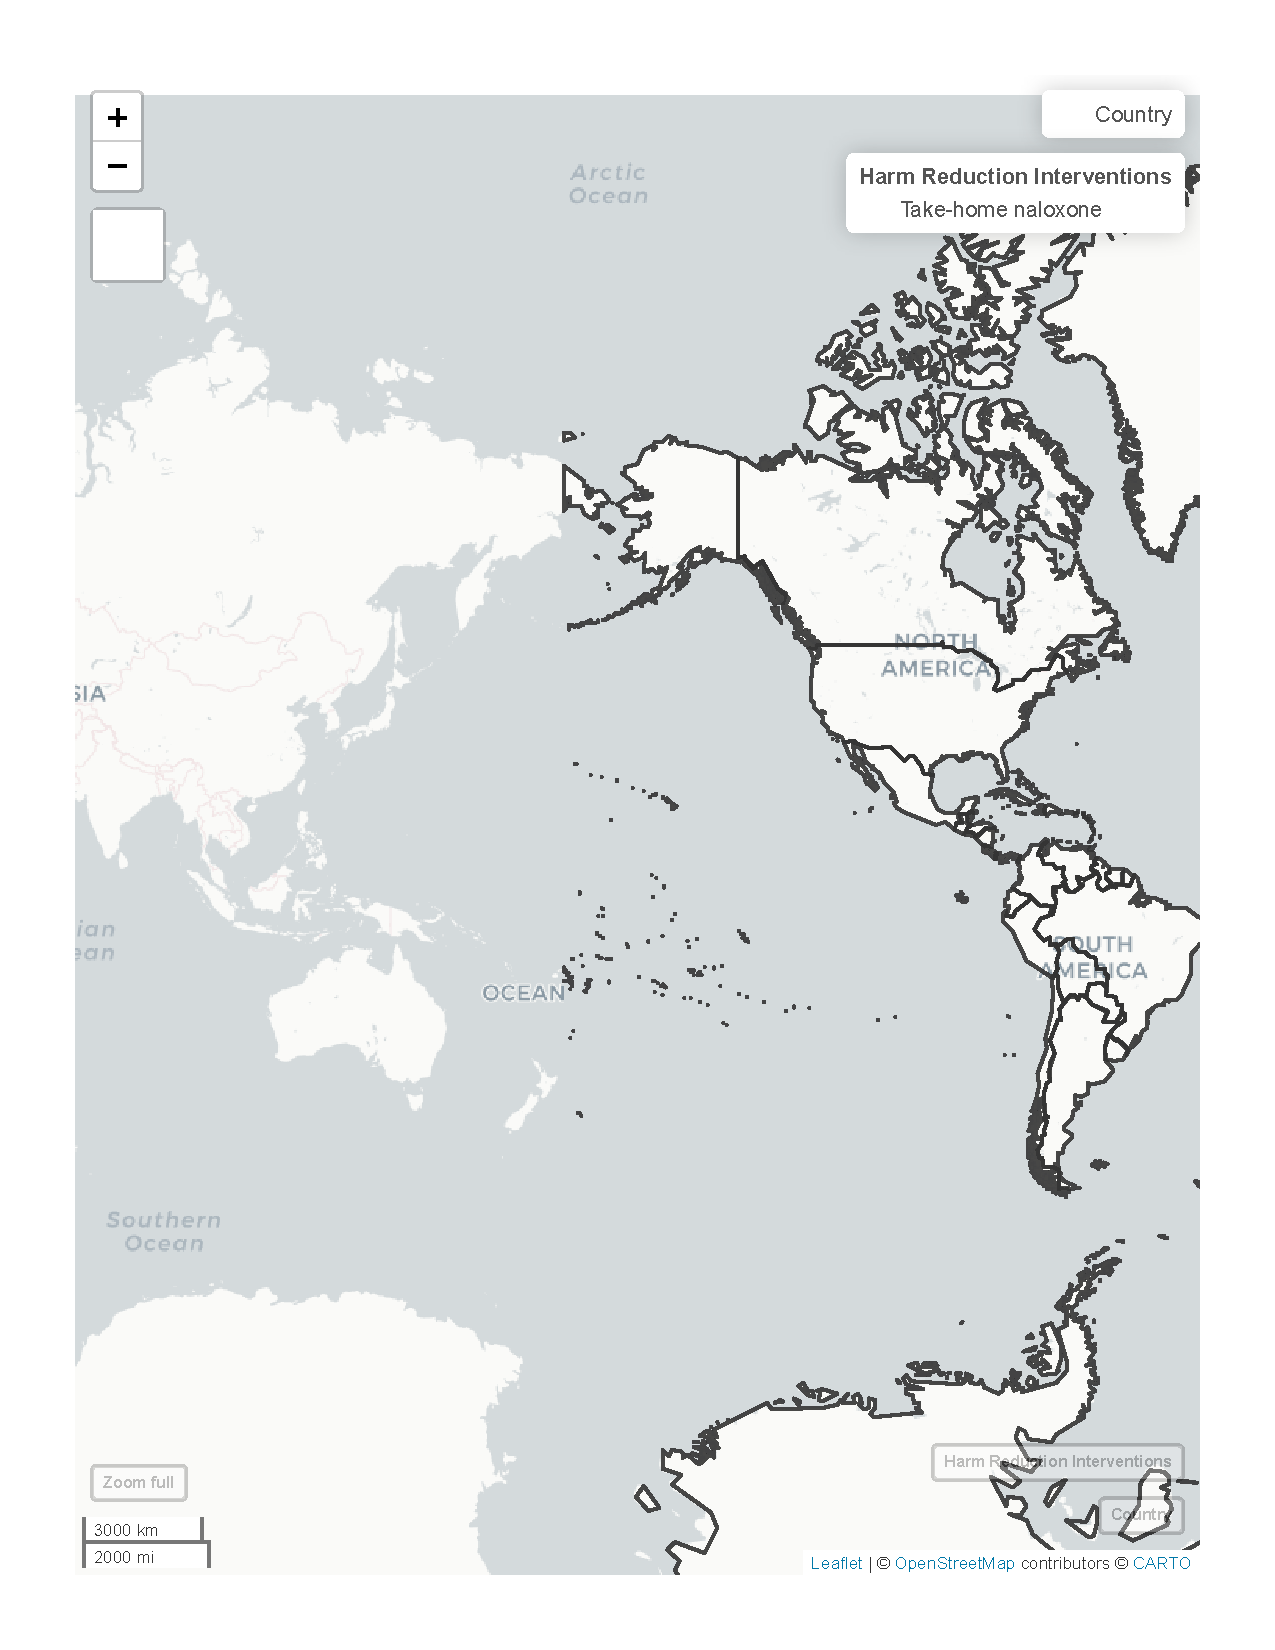
\includegraphics{index_files/figure-pdf/unnamed-chunk-2-1.pdf}

\textsubscript{Source:
\href{https://mx-jx.github.io/YPWUD/index-preview.html}{Article
Notebook}}

You can explore this map \href{map.html}{as its own web page here}

\pagebreak

\subsection{References}\label{references}

\singlespacing

\pagebreak

\phantomsection\label{refs}
\begin{CSLReferences}{1}{0}
\bibitem[\citeproctext]{ref-barratt2022}
Barratt, Monica J., and Fiona Measham. 2022. {``What Is Drug Checking,
Anyway?''} \emph{Drugs, Habits and Social Policy} 23 (3): 176--87.
\url{https://doi.org/10.1108/DHS-01-2022-0007}.

\bibitem[\citeproctext]{ref-bhandari2021}
Bhandari, Tulsi Ram, Bhushan Khatiwada, Bibika Rajbhandari, Amy Bestman,
Sabuj Kanti Mistry, Binod Rayamajhee, Lal B. Rawal, and Uday Narayan
Yadav. 2021. {``A Qualitative Study to Understand Drivers of
Psychoactive Substance Use Among Nepalese Youth.''} \emph{PLOS ONE} 16
(11): e0259021. \url{https://doi.org/10.1371/journal.pone.0259021}.

\bibitem[\citeproctext]{ref-brien2023}
Brien, Rita, Isabelle Volpe, Jasmin Grigg, Tom Lyons, Caitlin Hughes,
Ginny McKinnon, Stephanie Tzanetis, et al. 2023. {``Co-Designing Drug
Alerts for Health and Community Workers for an Emerging Early Warning
System in Victoria, Australia.''} \emph{Harm Reduction Journal} 20 (1):
30. \url{https://doi.org/10.1186/s12954-023-00761-6}.

\bibitem[\citeproctext]{ref-buxton2020}
Buxton, Julia. 2020. {``Drugs and Development: Drug Policies and the
Global South.''} In, 265--82. Edward Elgar Publishing.
\url{https://www.elgaronline.com/edcollchap/edcoll/9781788117050/9781788117050.00025.xml}.

\bibitem[\citeproctext]{ref-canuxeado2022}
Canêdo, Joana, Kali-olt Sedgemore, Kelly Ebbert, Haleigh Anderson,
Rainbow Dykeman, Katey Kincaid, Claudia Dias, et al. 2022. {``Harm
Reduction Calls to Action from Young People Who Use Drugs on the Streets
of Vancouver and Lisbon.''} \emph{Harm Reduction Journal} 19 (1): 43.
\url{https://doi.org/10.1186/s12954-022-00607-7}.

\bibitem[\citeproctext]{ref-chang2021}
Chang, Judy, Shaun Shelly, Machteld Busz, Claudia Stoicescu, Arif
Rachman Iryawan, Dinara Madybaeva, Yuri de Boer, and Andy Guise. 2021.
{``Peer Driven or Driven Peers? A Rapid Review of Peer Involvement of
People Who Use Drugs in HIV and Harm Reduction Services in Low- and
Middle-Income Countries.''} \emph{Harm Reduction Journal} 18 (1): 15.
\url{https://doi.org/10.1186/s12954-021-00461-z}.

\bibitem[\citeproctext]{ref-colledge-frisby2023}
Colledge-Frisby, Samantha, Sophie Ottaviano, Paige Webb, Jason Grebely,
Alice Wheeler, Evan B. Cunningham, Behzad Hajarizadeh, et al. 2023.
{``Global Coverage of Interventions to Prevent and Manage Drug-Related
Harms Among People Who Inject Drugs: A Systematic Review.''} \emph{The
Lancet Global Health} 11 (5): e673--83.
\url{https://doi.org/10.1016/S2214-109X(23)00058-X}.

\bibitem[\citeproctext]{ref-dambruoso2022}
D'Ambruoso, Lucia, Denny Mabetha, Rhian Twine, Maria van der Merwe,
Jennifer Hove, Gerhard Goosen, Jerry Sigudla, Sophie Witter, and On
behalf of the Verbal Autopsy with Participatory Action Research
(VAPAR)/Wits/Mpumalanga Department of Health Learning Platform. 2022.
{``{`}Voice Needs Teeth to Have Bite{'}! Expanding Community-Led
Multisectoral Action-Learning to Address Alcohol and Drug Abuse in Rural
South Africa.''} \emph{PLOS Global Public Health} 2 (10): e0000323.
\url{https://doi.org/10.1371/journal.pgph.0000323}.

\bibitem[\citeproctext]{ref-daniels2021}
Daniels, Colleen, Aggrey Aluso, Naomi Burke-Shyne, Kojo Koram, Suchitra
Rajagopalan, Imani Robinson, Shaun Shelly, Sam Shirley-Beavan, and
Tripti Tandon. 2021. {``Decolonizing Drug Policy.''} \emph{Harm
Reduction Journal} 18 (1): 120.
\url{https://doi.org/10.1186/s12954-021-00564-7}.

\bibitem[\citeproctext]{ref-david2023}
David, Ifeolu, Lisa Wegner, and Wilson Majee. 2023. {``{``}We Want to
See Youth That Would Be Better People Than Us{''}: A Case Report on
Addressing Adolescent Substance Use in Rural South Africa.''}
\emph{International Journal of Environmental Research and Public Health}
20 (4): 3493. \url{https://doi.org/10.3390/ijerph20043493}.

\bibitem[\citeproctext]{ref-debeck2017}
DeBeck, Kora, Tessa Cheng, Julio S. Montaner, Chris Beyrer, Richard
Elliott, Susan Sherman, Evan Wood, and Stefan Baral. 2017. {``HIV and
the Criminalisation of Drug Use Among People Who Inject Drugs: A
Systematic Review.''} \emph{The Lancet HIV} 4 (8): e357--74.
\url{https://doi.org/10.1016/S2352-3018(17)30073-5}.

\bibitem[\citeproctext]{ref-degenhardt2016}
Degenhardt, Louisa, Emily Stockings, George Patton, Wayne D. Hall, and
Michael Lynskey. 2016. {``The Increasing Global Health Priority of
Substance Use in Young People.''} \emph{The Lancet Psychiatry} 3 (3):
251--64. \url{https://doi.org/10.1016/S2215-0366(15)00508-8}.

\bibitem[\citeproctext]{ref-desjarlais2013}
Des Jarlais, Don C., Jonathan P. Feelemyer, Shilpa N. Modi, Abu
Abdul-Quader, and Holly Hagan. 2013. {``High Coverage Needle/Syringe
Programs for People Who Inject Drugs in Low and Middle Income Countries:
A Systematic Review.''} \emph{BMC Public Health} 13 (1): 53.
\url{https://doi.org/10.1186/1471-2458-13-53}.

\bibitem[\citeproctext]{ref-duxedazmoreno2022}
Díaz Moreno, Mauro, Nathalia Alarcón Ayala, Yarelix Estrada, Vannesa
Morris, and Julián Quintero. 2022. {``Échele Cabeza as a Harm Reduction
Project and Activist Movement in Colombia.''} \emph{Drugs, Habits and
Social Policy} 23 (3): 263--76.
\url{https://doi.org/10.1108/DHS-07-2022-0026}.

\bibitem[\citeproctext]{ref-doyle2022}
Doyle, Aoife M., Chido Dziva Chikwari, Nomathamsanqa Majozi, Musonda
Simwinga, Gracious R. Mayingire, Kelvin Simbeye, Stefanie Dringus, and
Sarah Bernays. 2022. {``Adolescent Health Series: Engagement with Young
People as Partners in Health Research: Four Case Studies from
Sub-Saharan Africa.''} \emph{Tropical Medicine \& International Health}
27 (1): 2--12. \url{https://doi.org/10.1111/tmi.13702}.

\bibitem[\citeproctext]{ref-duarte2020}
Duarte, Catherine d.P., Leslie Salas-Hernández, and Joseph S. Griffin.
2020. {``Policy Determinants of Inequitable Exposure to the Criminal
Legal System and Their Health Consequences Among Young People.''}
\emph{American Journal of Public Health} 110 (Suppl 1): S43--49.
\url{https://doi.org/10.2105/AJPH.2019.305440}.

\bibitem[\citeproctext]{ref-hall2016}
Hall, Wayne D., George Patton, Emily Stockings, Megan Weier, Michael
Lynskey, Katherine I. Morley, and Louisa Degenhardt. 2016. {``Why Young
People's Substance Use Matters for Global Health.''} \emph{The Lancet
Psychiatry} 3 (3): 265--79.
\url{https://doi.org/10.1016/S2215-0366(16)00013-4}.

\bibitem[\citeproctext]{ref-harker2020}
Harker, Nadine, Warren Covelé Lucas, Ria Laubscher, Siphokazi Dada,
Bronwyn Myers, and Charles DH Parry. 2020. {``Is South Africa Being
Spared the Global Opioid Crisis? A Review of Trends in Drug Treatment
Demand for Heroin, Nyaope and Codeine-Related Medicines in South Africa
(2012{\textendash}2017).''} \emph{International Journal of Drug Policy}
83 (September): 102839.
\url{https://doi.org/10.1016/j.drugpo.2020.102839}.

\bibitem[\citeproctext]{ref-harmreductioninternational2020}
Harm Reduction International. 2020. {``The Global State of Harm
Reduction 2020.''}
\url{https://hri.global/wp-content/uploads/2022/10/Global_State_HRI_2020_BOOK_FA_Web-1.pdf}.

\bibitem[\citeproctext]{ref-hernuxe1ndezcastillo2019}
Hernández Castillo, Rosalva Aída. 2019. {``Racialized Geographies and
the {``}War on Drugs{''}: Gender Violence, Militarization, and
Criminalization of Indigenous Peoples.''} \emph{The Journal of Latin
American and Caribbean Anthropology} 24 (3): 635--52.
\url{https://doi.org/10.1111/jlca.12432}.

\bibitem[\citeproctext]{ref-idpc2021}
IDPC. 2021. {``Human Rights and Drug Policies in Nepal.''}
\url{https://idpc.net/publications/2021/12/human-rights-and-drug-policies-in-nepal}.

\bibitem[\citeproctext]{ref-jacobs2020}
Jacobs, Wura, Ann O Amuta-Jimenez, Olufunto A. Olusanya, Alane Fajayan
Bristow, Davies Adeloye, and Adam E. Barry. 2020. {``Socio-Ecological
Factors of Adolescent Substance Use in Nigeria: A Systematic Review of
Literature.''} \emph{Journal of Health Care for the Poor and
Underserved} 31 (4): 1765--84.
\url{https://muse.jhu.edu/pub/1/article/772771}.

\bibitem[\citeproctext]{ref-jumbe2021}
Jumbe, Sandra, Tony Mwenda Kamninga, Isaac Mwalwimba, and Ukwuori-Gisela
Kalu. 2021. {``Determinants of Adolescent Substance Use in Africa: A
Systematic Review and Meta-Analysis Protocol.''} \emph{Systematic
Reviews} 10 (1): 125. \url{https://doi.org/10.1186/s13643-021-01680-y}.

\bibitem[\citeproctext]{ref-kakchapati2018}
Kakchapati, Sampurna, Bishnu Shrestha, Dan Y Li, Rajesh Rajbhandari, and
Tarun Poudel. 2018. {``Drug Use, Injecting Behaviors, and Survival Sex
Among Street Children and Youths in Kathmandu Valley, Nepal.''}
\emph{International Journal of STD \& AIDS} 29 (6): 588--97.
\url{https://doi.org/10.1177/0956462417746532}.

\bibitem[\citeproctext]{ref-kimmel2020}
Kimmel, Simeon D., Alexander Y. Walley, Yijing Li, Benjamin P. Linas,
Sara Lodi, Dana Bernson, Roger D. Weiss, Jeffrey H. Samet, and Marc R.
Larochelle. 2020. {``Association of Treatment with Medications for
Opioid Use Disorder with Mortality After Hospitalization for Injection
Drug Use{\textendash}associated Infective Endocarditis.''} \emph{JAMA
Network Open} 3 (10): e2016228.
\url{https://doi.org/10.1001/jamanetworkopen.2020.16228}.

\bibitem[\citeproctext]{ref-krug2012}
Krug, Anita. 2012. {``A Global Review of Harm Reduction Services for
Young People.''}

\bibitem[\citeproctext]{ref-krug2015}
Krug, Anita, Mikaela Hildebrand, and Nina Sun. 2015. {``{``}We Don't
Need Services. We Have No Problems{''}: Exploring the Experiences of
Young People Who Inject Drugs in Accessing Harm Reduction Services.''}
\emph{Journal of the International AIDS Society} 18 (2S1): 19442.
\url{https://doi.org/10.7448/IAS.18.2.19442}.

\bibitem[\citeproctext]{ref-lambdin2013}
Lambdin, Barrot H., R. Douglas Bruce, Olivia Chang, Cassian Nyandindi,
Norman Sabuni, Sophia Zamudio-Haas, Sheryl McCurdy, et al. 2013.
{``Identifying Programmatic Gaps: Inequities in Harm Reduction Service
Utilization Among Male and Female Drug Users in Dar Es Salaam,
Tanzania.''} \emph{PLOS ONE} 8 (6): e67062.
\url{https://doi.org/10.1371/journal.pone.0067062}.

\bibitem[\citeproctext]{ref-morales2020}
Morales, Mario, Claudia Rafful, Pieter Baker, Jaime Arredondo, Sunyou
Kang, Maria L. Mittal, Teresita Rocha-Jiménez, Steffanie A. Strathdee,
and Leo Beletsky. 2020. {``{``}Pick up Anything That Moves{''}: A
Qualitative Analysis of a Police Crackdown Against People Who Use Drugs
in Tijuana, Mexico.''} \emph{Health \& Justice} 8 (1): 9.
\url{https://doi.org/10.1186/s40352-020-00111-9}.

\bibitem[\citeproctext]{ref-ogundipe2018}
Ogundipe, O., E. O. Amoo, D. Adeloye, and -Isaac A. Olawole. 2018.
{``Substance Use Among Adolescents in Sub-Saharan Africa : A Systematic
Review and Meta-Analysis.''} \emph{South African Journal of Child
Health} 2018 (1): s79--84.
\url{https://doi.org/10.7196/SAJCH.2018.v12i2.1524}.

\bibitem[\citeproctext]{ref-pauly2008}
Pauly, Bernadette. 2008. {``Harm Reduction Through a Social Justice
Lens.''} \emph{International Journal of Drug Policy}, Values and ethics
in harm reduction, 19 (1): 4--10.
\url{https://doi.org/10.1016/j.drugpo.2007.11.005}.

\bibitem[\citeproctext]{ref-peltzer2018}
Peltzer, Karl, and Nancy Phaswana-Mafuya. 2018. {``Drug Use Among Youth
and Adults in a Population-Based Survey in South Africa.''} \emph{The
South African Journal of Psychiatry : SAJP : The Journal of the Society
of Psychiatrists of South Africa} 24 (April): 1139.
\url{https://doi.org/10.4102/sajpsychiatry.v24i0.1139}.

\bibitem[\citeproctext]{ref-rekart2005}
Rekart, Michael L. 2005. {``Sex-Work Harm Reduction.''} \emph{The
Lancet} 366 (9503): 2123--34.
\url{https://doi.org/10.1016/S0140-6736(05)67732-X}.

\bibitem[\citeproctext]{ref-scheibe2020}
Scheibe, Andrew, Shaun Shelly, and Anna Versfeld. 2020.
{``Prohibitionist Drug Policy in South Africa{\textemdash}Reasons and
Effects.''} \emph{International Development Policy \textbar{} Revue
Internationale de Politique de Développement}, no. 12 (September).
\url{https://doi.org/10.4000/poldev.4007}.

\bibitem[\citeproctext]{ref-scheim2020}
Scheim, Ayden I., Nazlee Maghsoudi, Zack Marshall, Siobhan Churchill,
Carolyn Ziegler, and Dan Werb. 2020. {``Impact Evaluations of Drug
Decriminalisation and Legal Regulation on Drug Use, Health and Social
Harms: A Systematic Review.''} \emph{BMJ Open} 10 (9): e035148.
\url{https://doi.org/10.1136/bmjopen-2019-035148}.

\bibitem[\citeproctext]{ref-serebryakova2021}
Serebryakova, Lela, Catherine Cook, and Charlotte Davies. 2021. {``The
Continued Crisis for Harm Reduction Funding in Low- and Middle-Income
Countries.''} \emph{Harm Reduction International}.

\bibitem[\citeproctext]{ref-stockings2016}
Stockings, Emily, Wayne D Hall, Michael Lynskey, Katherine I Morley,
Nicola Reavley, John Strang, George Patton, and Louisa Degenhardt. 2016.
{``Prevention, Early Intervention, Harm Reduction, and Treatment of
Substance Use in Young People.''} \emph{The Lancet Psychiatry} 3 (3):
280--96. \url{https://doi.org/10.1016/S2215-0366(16)00002-X}.

\bibitem[\citeproctext]{ref-stowe2022}
Stowe, M-J, Orsi Feher, Beatrix Vas, Sangeet Kayastha, and Alissa Greer.
2022. {``The Challenges, Opportunities and Strategies of Engaging Young
People Who Use Drugs in Harm Reduction: Insights from Young People with
Lived and Living Experience.''} \emph{Harm Reduction Journal} 19 (1):
83. \url{https://doi.org/10.1186/s12954-022-00663-z}.

\bibitem[\citeproctext]{ref-tinasti2018}
Tinasti, Khalid. 2018. {``HIV and AIDS Among Adolescents Who Use Drugs:
Opportunities for Drug Policy Reform Within the Sustainable Development
Agenda.''} \emph{Journal of the International AIDS Society} 21 (S1):
e25045. \url{https://doi.org/10.1002/jia2.25045}.

\bibitem[\citeproctext]{ref-delatorre-luque2021}
Torre-Luque, Alejandro de la, Fatos Ozeylem, and Cecilia A. Essau. 2021.
{``Prevalence of Addictive Behaviours Among Adolescents from 73 Low-and
Middle-Income Countries.''} \emph{Addictive Behaviors Reports} 14
(December): 100387. \url{https://doi.org/10.1016/j.abrep.2021.100387}.

\bibitem[\citeproctext]{ref-toumbourou2007}
Toumbourou, J. W., T. Stockwell, C. Neighbors, G. A. Marlatt, J. Sturge,
and J. Rehm. 2007. {``Interventions to Reduce Harm Associated with
Adolescent Substance Use.''} \emph{The Lancet} 369 (9570): 1391--401.
\url{https://doi.org/10.1016/S0140-6736(07)60369-9}.

\bibitem[\citeproctext]{ref-unodc2022}
UNODC. 2022. {``World Drug Report 2022.''}
\href{https:////www.unodc.org/unodc/en/data-and-analysis/wdr-2022_booklet-2.html}{//www.unodc.org/unodc/en/data-and-analysis/wdr-2022\_booklet-2.html}.

\bibitem[\citeproctext]{ref-wodak2012}
Wodak, Alex. 2012. {``Drug Law Reform: When Bad Policy Is Good
Politics.''} \emph{The Lancet} 380 (9854): 1624--26.
\url{https://doi.org/10.1016/S0140-6736(12)61847-9}.

\bibitem[\citeproctext]{ref-worldhealthorganization2009}
World Health Organization, World Health Organization. Regional Office
for Europe, UNAIDS, United Nations. Office on Drugs, and Crime. 2009.
{``WHO, UNODC, UNAIDS Technical Guide for Countries to Set Targets for
Universal Access to HIV Prevention, Treatment and Care for Injecting
Drug Users.''} \emph{OMS, ONUDC, ONUSIDA : Guide Technique Destiné Aux
Pays Pour La Définition Des Objectifs Nationaux Pour l'accès Universel à
La Prévention, Au Traitement, Aux Soins Et Au Soutien En Matière de
VIH/SIDA}, 40. \url{https://iris.who.int/handle/10665/44068}.

\bibitem[\citeproctext]{ref-zampini2018}
Zampini, Giulia Federica. 2018. {``Evidence and Morality in
Harm-Reduction Debates: Can We Use Value-Neutral Arguments to Achieve
Value-Driven Goals?''} \emph{Palgrave Communications} 4 (1): 1--10.
\url{https://doi.org/10.1057/s41599-018-0119-3}.

\end{CSLReferences}



\end{document}
